\documentclass[a4paper,14pt]{article}
\usepackage{float}
\usepackage{extsizes}
\usepackage{amsmath}
\usepackage{amssymb}
\everymath{\displaystyle}
\usepackage{geometry}
\usepackage{fancyhdr}
\usepackage{multicol}
\usepackage{graphicx}
\usepackage[brazil]{babel}
\usepackage[shortlabels]{enumitem}
\usepackage{cancel}
\usepackage{textcomp}
\usepackage{array} % Para melhor formatação de tabelas
\usepackage{longtable}
\usepackage{booktabs}  % Para linhas horizontais mais bonitas
\usepackage{float}   % Para usar o modificador [H]
\usepackage{caption} % Para usar legendas em tabelas
\usepackage{tcolorbox}

\columnsep=2cm
\hoffset=0cm
\textwidth=8cm
\setlength{\columnseprule}{.1pt}
\setlength{\columnsep}{2cm}
\renewcommand{\headrulewidth}{0pt}
\geometry{top=1in, bottom=1in, left=0.7in, right=0.5in}

\pagestyle{fancy}
\fancyhf{}
\fancyfoot[C]{\thepage}

\begin{document}
	
	\noindent\textbf{6FMA51 - Matemática} 
	
	\begin{center}Diagrama de Venn e intersecção de conjuntos (Versão estudante)
	\end{center}
	
	\noindent\textbf{Nome:} \underline{\hspace{10cm}}
	\noindent\textbf{Data:} \underline{\hspace{4cm}}
	
	%\section*{Questões de Matemática}
	\begin{multicols}{2}
    		\noindent Para representar conjuntos, utilizamos o diagrama de Venn. Neste, o conjunto universo é representado por um retângulo e cada conjunto é representado por uma curva que não corta a si mesma, geralmente uma circunferência. \\
    		A intersecção de dois conjuntos $A$ e $B$ (que simbolizamos por $A \cap B$) é formada pelos elementos que pertencem a $A$ e pertencem a $B$. \\
    		Se a intersecção de dois conjuntos é vazia, dizemos que eles são disjuntos.
    		\textsubscript{---------------------------------------------------------------------}
    		\begin{enumerate}
    			\item Sendo $U = \{1, 2, 3, 4, 5, 6, 7, 8, 9, 10\}$, utilizando diagramas de Venn, representar os pares de conjuntos:
    			\begin{enumerate}[a)]
    				\item $A = \{1, 2, 3, 4, 5\}, \\ B = \{1, 2, 4, 6, 7, 9\}$ \\\\\\\\\\\\\\\\\\\\\\\\\\\\
    				\item $A = \{1, 2, 3, 4, 5, 8, 10\}, B = \{2, 8, 10\}$ \\\\\\\\\\\\\\\\\\\\\\
    				\item $A = \{3, 5, 7, 9\}, B = \{1, 2, 3, 5, 7, 8, 9, 10\}$ \\\\\\\\\\\\\\\\\\\\\\
    				\item $A = \{3, 4, 6, 7, 9\}, \\ B = \{3, 4, 6, 7, 9\}$ \newpage
    				\item $A = \{1, 3, 5, 7\}, \\ B = \{2, 4, 6, 10\}$ \\\\\\\\\\\\\\\\\\\\\\
    			\end{enumerate}
    			\item Dados $A$ e $B$, apresentar $A \cap B$.
    				\begin{enumerate}[a)]
    				\item $A = \{2, 4, 6\}, B = \{2, 1\}$ \\\\\\\\\\\\\\\\\\\\\\
    				\item $A =\{1, 2, 3\}, B = {2, 3}$ \\\\\\\\\\\\\\\\\\\\\\\\
    				\item $A = \{6, 7\}, B = \{6, 7\}$ \\\\\\\\\\\\\\\\\\\\\\
    				\item $A = \varnothing, B = \varnothing$ \\\\\\\\\\\\\\\\\\\\\\
    				\end{enumerate}
    				\item Dados $X, Y$ e $Z$, apresentar \\ $X \cap Y \cap Z$.
    				\begin{enumerate}[a)]
    					\item $X = \{3, 4, 5\}, \\ Y = \{4, 5, 6\}, \\ Z = \{5, 6, 7\}$ \\\\\\\\\\\\\\\\\\\\
    					\item $X = \{6, 7, 8\}, \\ Y = \{8, 9 ,10\}, \\ Z = \{10, 11, 12\}$ \columnbreak
    				\end{enumerate}
    				\item Hachurar $A \cap B$ \\
    				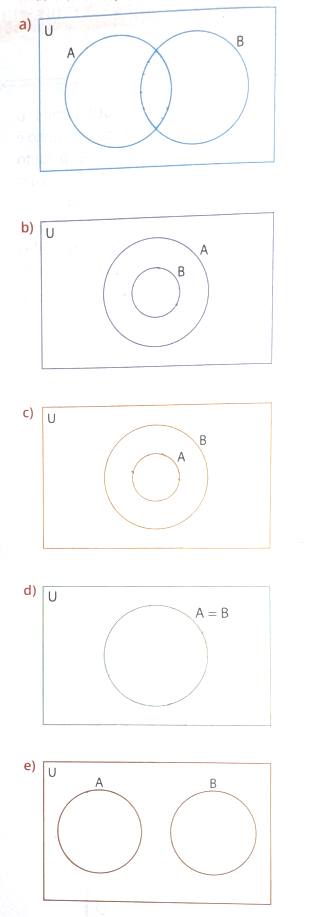
\includegraphics[width=1\linewidth]{imagens_6FMA51/imagem1}
    				\newpage
    				\item Assinale \textbf{V} (verdadeiro) ou \textbf{F} (falso).
    				\begin{enumerate}[a)]
    					\item $5 + 1 = 6 \land 7 - 3  = 4$
    					\item $3 + 5 = 7$ e $8 - 2 = 6$
    					\item $4 + 5 = 9 \lor 6 - 5 = 2$
    					\item $7 - 6 = 2$ ou $4 + 5 = 9$
    					\item $\frac{1}{3} = \frac{3}{9} \land 12 \cdot 2 = 6 \cdot 4$
    					\item $\frac{1}{5} = \frac{1}{10} \lor 3 \cdot 4 = 6 \cdot 3$
    					\item 7 é par e 8 é ímpar
    					\item 3 é ímpar ou 6 é par
    				\end{enumerate}
    				\item Dados $A$ e $B$, apresentar $A \cap B$:
    				\begin{enumerate}[a)]
    					\item $A = \{1, 2, 3\}, B = \{1, 2\}$
    					\item $A = \{2, 4, 6\}, B = \{4, 5\}$
    					\item $A = \{10, 11\}, B = \{10, 11\}$
    					\item $A = \{\varnothing, 5\}, B = \varnothing$
    					\item $A = \{1, \{2\}, 3, 4\}, \\ B = \{\{2\}, \{3\}\}$
    					\item $A = \{1, \{1\}\}, B = \{5, 6, 7\}$
    					\item $A = \varnothing, B = \{5, 6, 7\}$
    					\item $A = \{\varnothing\}, B = \{\{\varnothing\}\}$
    				\end{enumerate}
    				\item Sendo $U = \{5, 6, 7, 8, 9, 10, 11, 12, 13\}$, utilizando diagramas de Venn, representar as partes de conjuntos e apresentar $A \cap B$:
    				\begin{enumerate}[a)]
    					\item $A = \{5, 6, 7\}, \\ B = \{6, 7, 8, 10, 11\}$
    					\item $A = \{8, 9\}, B = \{8, 9, 10, 11\}$
    					\item $A = \{10, 11, 12, 13\}, \\ B = \{10, 11\}$
    					\item $A = \{8, 9, 10, 11\}, \\ B = \{5, 6, 12\}$
    				\end{enumerate}
    				\item Dados $X, Y$ e $Z$, apresentar $X \cap Y \cap Z$:
    				\begin{enumerate}[a)]
    					\item $X = \{21, 22, 23\}, \\ Y = \{22, 23\}, \\ Z = \{23, 24, 25\}$
    					\item $X = \{\varnothing, 5\}, \\ Y = \{\{\varnothing\}, \varnothing\}, \\ Z = \{\varnothing, 4, 6\}$
    					\item $X = \{8, 9\}, Y = \{9, 10\}, \\ Z = \{10, 11\}$
    					\item $X = \{15, 16\}, \\ Y = \{15, 16, 17, 18\}, \\ Z = \{14, 15, 16\}$ 
    				\end{enumerate}
    				\item Hachurar $A \cap B \cap C$.
    				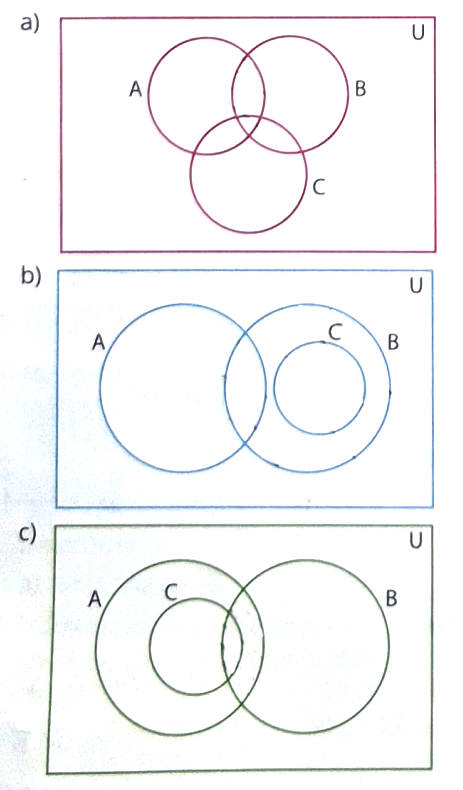
\includegraphics[width=1\linewidth]{imagens_6FMA51/imagem2}
    				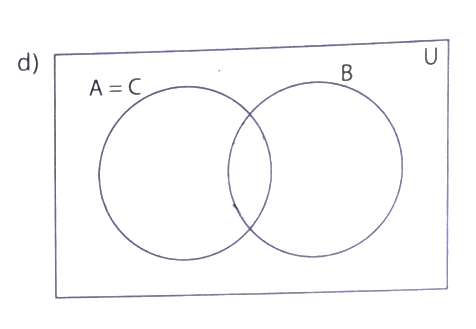
\includegraphics[width=1\linewidth]{imagens_6FMA51/imagem3}
    				
    			\end{enumerate}
    			$~$ \\ $~$ \\ $~$ \\ $~$ \\ $~$ \\ $~$ \\ $~$ \\ $~$ \\ $~$ \\ $~$ \\ $~$ \\ $~$ \\ $~$ \\ $~$ \\ $~$ \\ $~$ \\ $~$ \\ $~$ \\ $~$ \\ $~$ \\ $~$ \\ $~$ \\ $~$ \\ $~$ \\ $~$ \\ $~$ \\ $~$ \\ $~$ \\ $~$ \\ $~$ \\ $~$ \\ $~$ \\ $~$ \\ $~$ \\ $~$ \\ $~$ \\ $~$ \\ $~$ \\ $~$ \\ $~$ \\ $~$ \\ $~$ \\ $~$ \\ $~$ \\ $~$ \\ $~$ \\ $~$ \\ $~$ \\ $~$ \\ $~$ \\ $~$ \\ $~$ \\ $~$ \\ $~$ \\ $~$ \\ $~$ \\ $~$ \\ $~$ \\ $~$ \\ $~$ \\ $~$ \\ $~$ \\ $~$ \\ $~$ \\ $~$ \\ $~$ \\ $~$ \\ $~$ \\ $~$ \\ $~$ \\ $~$ \\ $~$ \\ $~$ \\ $~$ \\ 
	\end{multicols}
\end{document}